\chapter{Evaluation}
\label{cha:eval}
This research project has among its main aims the evaluation of results, described in this chapter. It is important to analyse how this general purpose application performs under the SpiNNaker environments and what architectural limitations it faces, which is useful feedback to the team. The chapter outlines also performance benchmarks of SpiDB in comparison with other database systems and how it can be improved.

\section{Transmission delay}
\label{sec:eval_comm_rel}

According to my experiments, sending SDP packets immediately between two cores results on a very large packet drop ration. Without explicit delay between the transmission of packets, the number of successful deliveries is only about 10\% of those sent for a large number of packets. This effect is strongly reduced by the addition of a small delay of 5-10$\mu$s, which guarantees over 99\% successful deliveries, as can be seen on table \ref{table:sdp_deliveries}. The table also shows that having long delays, greater than 10$\mu$s is mostly redundant, as they do not decrease packet loss significantly, but tragically reduce throughput.

Upon experimenting, I found that sending a large amount of consecutive, immediate packets (at least 1,000,000) has a chance of consequently crashing the destination core or causing it to reach the erraneous watchdog state (WDOG), meaning it cannot respond to commands.

\begin{table}
\begin{tabular}{ r | c | c | c | c | c }
 & \multicolumn{5}{c}{\textbf{Successful deliveries (\%)}} \\

\textbf{Packets sent} & \textbf{no delay} & \textbf{2$\mu$s delay} & \textbf{5$\mu$s delay} & \textbf{10$\mu$s delay} & \textbf{100$\mu$s delay} \\
50,000 & 9.56\% & 57.73\% & 95.95\% & 98.36\% & 99.85\% \\
100,000 & 12.15\% & 54.97\% & 97.99\% & 99.13\% & 99.92\% \\
200,000 & 13.07\% & 50.55\% & 99.01\% & 99.33\% & 99.96\% \\
500,000 & 12.97\% & 50.08\% & 99.49\% & 99.80\% & 99.99\% \\
1,000,000 & 13.05\% & 45.06\% & 98.84\% & 99.88\% & 99.99\% \\
\end{tabular}
\caption{Successful SDP deliveries with delay between each packet}
\label{table:sdp_deliveries}
\end{table}

Note that the experiment, made on SpiNN-3, involved sending a single SDP packet multiple times to the same destination on the same chip, containing only the 8 byte SDP header. The destination did not store or read the packet contents, only incrementing a counter upon packet receival. This was used to show the maximum possible transmission rate allowed by the SDP protocol under the hardware communication fabric. Code snippets and more information can be found on the appendix under the appendix section \ref{sec:appendix_comm_rel}.

Ideally these packets would send useful information, to be read upon arrival, which would keep the destination busy. From my experience and input from the team, the best way to achieve this is by immediately storing the SDP packet contents into a buffer when it is received and then handling it at a different point in time (listing \ref{lst:sdp_packet_callback}). The reason for this is that if another packet arrives as we are processing the current packet with same or higher priority, the incomming packet will drop.

High priority should be assigned to storing incomming packets into a buffer and the actual processing should have lower priority, as it can be handled at a later point in time. It is important to note that this can cause starvation and buffer overflow if there are too many immediate packets being received. For instance, if our SDP packet is of size 12-byte (8-byte header + 32-bit data) and stored into a buffer in private DTCM memory upon receival, we would only ever be able to hold up to about 5,000 messages at once (64-Kbytes DTCM size / 12-byte packet size). Realistically a large part of DTCM contains the stack, local and global variables, so that number will be drastically reduced. In my application, SpiDB, insert and retrieve database queries have a size of 256-bytes, which means a limit of 250 entries in the buffer if memory were empty.

This evaluation is important because it allows finding the optimal transmission delay for an application. A developer on SpiNNaker using the point-to-point protocol needs to find the balance between transmission rate and reliability, which are inversely proportional. This balance is application dependent.

\lstinputlisting[language=C, caption=Storing incomming packets into a queue, label={lst:sdp_packet_callback}]{code/sdp_packet_callback.c}

On SpiDB, I experimented with different time delays when transmitting packets from host over ethernet to a core on SpiNNaker, in order to find the best evaluation. The speed of one operation is calculated as the time of successful reply minus the time that operation was sent from host, thus being a round-trip-time plus internal processing time. The performance is calculated as the amount of operations successfully executed in one second.

As can be seen on figure \ref{fig:transmission-delay}, large packet transmission delays of 50-100$\mu$s are redundant, as they do not reduce packet drops, while being a high cost on performance. Naturally the more packets we can send in one second influences the speed of replies, thus improving performance. This hits a maxima at 40$\mu$s, with almost 10,000 op/sec, in which transmission is at a high rate with no loss of reliability. Transmission delays between 40-10$\mu$s result on a decrease of performance, because although packets are sent more frequently, a lot of them are dropped (up to about 35\%), being also extremely unreliable. We reach the worst case at 10-5$\mu$s delay, when the destination core cannot cope with the speed of incomming packets, simply crashing and ceasing to respond. This SpiDB experiment was performed with 100,000 \textit{put} operations with keys and values of size 4-bytes each. More information on the data gathered can be found on the appendix under section \ref{sec:appendix_comm_rel}.

\begin{figure}
\begin{center}
	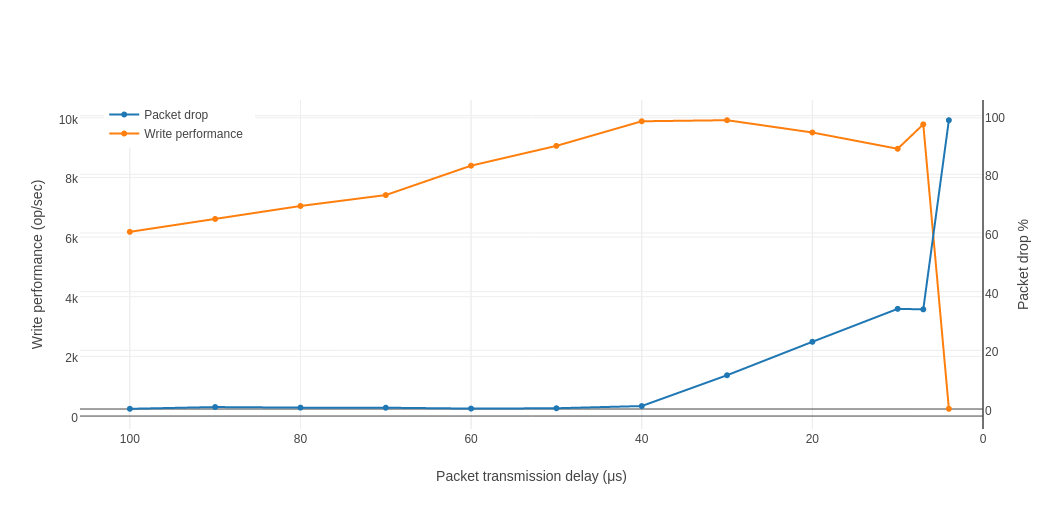
\includegraphics[width=1.4\textwidth, natwidth=1063, natheight=509]{images/transmission_delay.png}
\end{center}
\caption{Transmission delay plot}
\label{fig:transmission-delay}
\end{figure}

%what are reasons for packets to drop? because thingy just takes 1 microsecond or does it?...

\section{Performance benchmark}

\iffalse
In order to evaluate the performance of my database management system, I compared it with two of the most popular RAM-based Key-value pair databases: \textbf{memcached} and \textbf{Redis}.

Figure \ref{fig:write-perf-benchmark} shows a plot of the performance of the SpiNNaker Database (SpiDB) against these competitors for 100,000 consecutive \textit{put} operations. It can be seen that SpiDB runs at about 7,000-8,000 operations per second, which is slower than the others by a factor of 8. Performance for all systems was mostly constant given input size, up to the maximum \textit{SDP} data size of 256-bytes. The specifications can be found at appendix under section \ref{sec:appendix-specs}.

how to improve this? spinnlink

scalability:
THIS TAKES 1microsecond using the watchdog timer.

response times. why are they so high sometimes?!?!
first explain how we gather the time (operating system could be interrupting, sark, etc.)
This would ideally allow a linear speedup of data retrival in comparison with a sequential system.

100,000



\begin{figure}
\begin{center}
	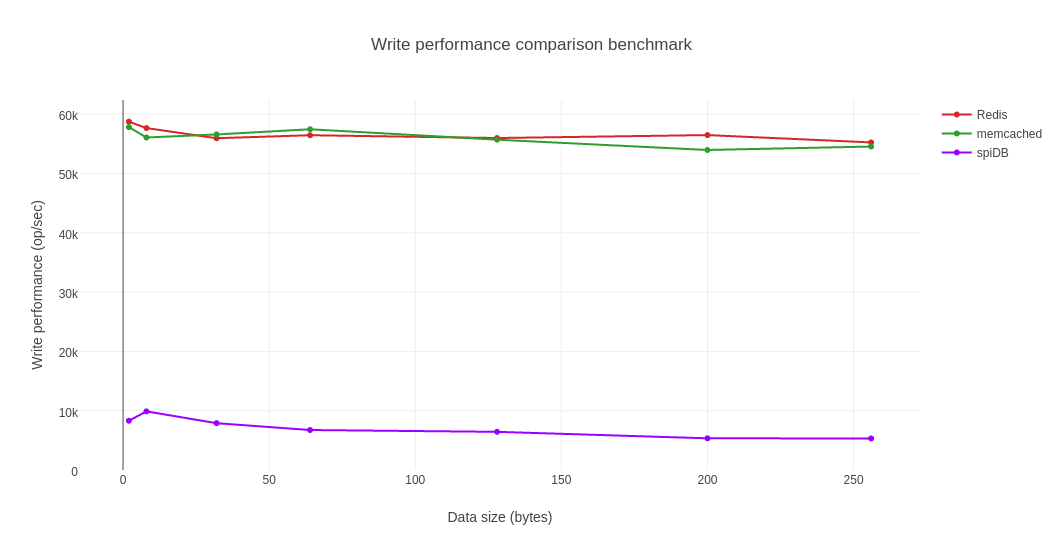
\includegraphics[width=1.4\textwidth, natwidth=1063, natheight=509]{images/write_performance.png}
\end{center}
\caption{PUT operation performance benchmark}
\label{fig:write-perf-benchmark}
\end{figure}
\fi


(still needs writting)

%\section{Hash vs Naive}

%\section{Sequential vs Parallel}

\section{Limitations}

(still needs writting)

%-SDRAM bandwidth
%-single point of failure for each board(mention that it is already like that. no way to avoid).
%-no global timer (gathering performance info...)

\iffalse

\begin{figure}
\begin{center}
	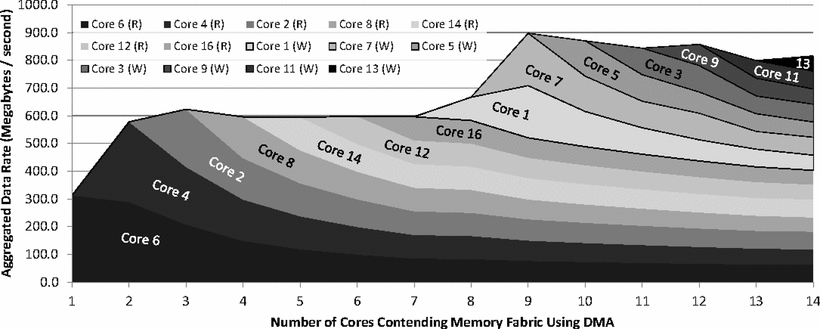
\includegraphics[width=1.2\textwidth, natwidth=820, natheight=329]{images/sdram_bandwidth.png}
\end{center}
\caption{SDRAM bandwidth utilization}
\label{fig:write-perf-benchmark}
\end{figure}

\fi

\section{Future work}
This project has been the tip of the iceberg of what a fully-functional SpiNNaker database management system can be, involving mostly research and simple operations to evaluate its performance. All code written by me is now part of the official open-source SpiNNaker API, available to the team and any developers interested. This means SpiDB is likely to expand in the future or serve as an example application running on SpiNNaker, accessible to researchers around the globe.

These are some features which can be implemented or improved in the future:

\begin{itemize}
	\item \textbf{Caching} and \textbf{indexing}: frequently accessed areas of shared SDRAM memory could be cached at the smaller but much faster private DTCM.
	\item \textbf{Security} and \textbf{multi-user access}: different sections of the database can have restricted access through credentials checking.
	\item \textbf{Scalability testing} on the large scale million core machine.
	\item An application \textbf{server} allowing queries to be requested over the internet on different locations.
	\item Improve \textbf{reliability} and increase \textbf{query sizes}, perhaps by implementing a protocol on top of the \textit{SDP} and \textit{MC} layer. As of now packets are limited to 256-bytes, with unreliability during busy times.
	\item \textbf{Self balancing} during idle times. While no queries are being executed, cores could distribute their contents in a balanced way for faster retrival. Indexing or other pre-processing could also be executed on the meantime.
	\item \textbf{Additional operations} supporting table merges, triggers and aggregations.
\end{itemize}